\documentclass{article}

\usepackage{graphicx}
\usepackage[hidelinks]{hyperref}
\usepackage[a4paper, total={6in, 8in}]{geometry}
\usepackage[slovak]{babel}
\usepackage{caption}
\usepackage{subcaption}

\graphicspath{./include/}

\renewcommand{\figurename}{Obr.}
\renewcommand{\contentsname}{Obsah}

\begin{document}

\begin{titlepage}
	\null\vfill

	\begin{center}
		{\Huge Regulácia výšky hladiny }
		\vskip 2cm

		{\Large Cvičenie č. 10}
		\vskip 0.5cm

		{\large Spojité procesy}
	\end{center}

	\vfill
	\vfill

	\begin{flushright}
		Filip Lobpreis \\
		Matúš Machata \\
		\small\today\\
	\end{flushright}
	\hfill
\end{titlepage}

\thispagestyle{empty}
\clearpage

\tableofcontents
\thispagestyle{empty}
\clearpage

\section{Zadanie}
\label{sec:zadanie}
\pagenumbering{arabic}

\begin{figure}[!htbp]
	\begin{center}
		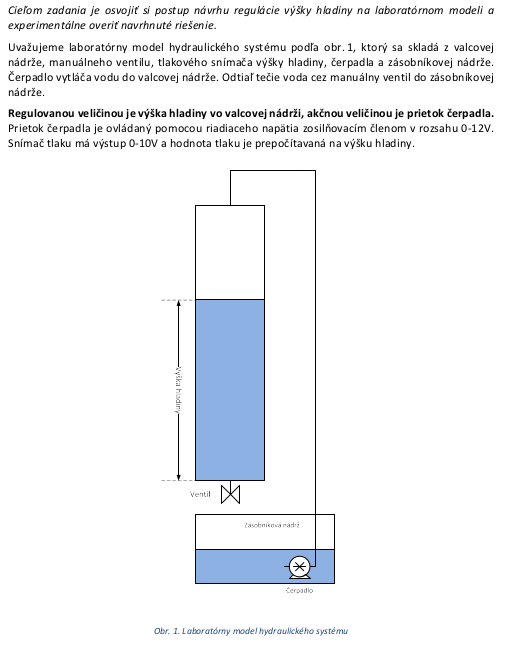
\includegraphics[width=0.8\textwidth]{./include/zadaniep1.png}
	\end{center}
	\caption{Prvá časť zadania z~cvičenia č. 9 z~predmetu spojité procesy}
	\label{fig:zadanie1}
\end{figure}

\begin{figure}[!htbp]
	\begin{center}
		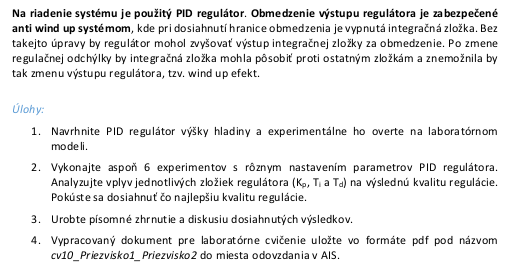
\includegraphics[width=0.8\textwidth]{./include/zadaniep2.png}
	\end{center}
	\caption{Druhá časť zadania z~cvičenia č. 9 z~predmetu spojité procesy}
		\label{fig:zadanie2}
\end{figure}

\clearpage

\section{Pomôcky}
\label{sec:pomocky}

V~tomto zadaní je našou úlohou experimentálne overiť návrh regulácie výšky hladiny na~laboratórnom
modeli hydraulického systému a~overiť navrhované riešenie. Pri~tomto zadaní sme použili už~preddefinovanú schému
v~programe \textit{Simulink} (Obr.~\ref{fig:schema}).

\begin{figure}[!htbp]
	\begin{center}
		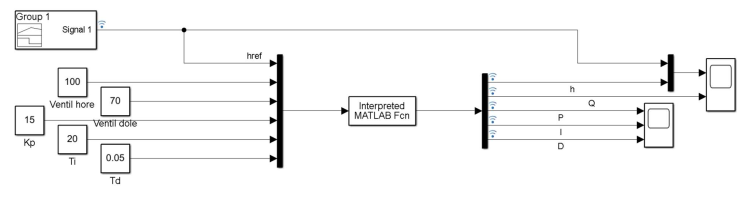
\includegraphics[width=0.8\textwidth]{./include/schema.png}
	\end{center}
	\caption{Schéma modelu z~cvičenia č. 9 z~predmetu spojité procesy}
	\label{fig:schema}
\end{figure}

V~tomto zapojení vidíme viacero vstupnych signálov, tie sú už~preddefinované. \textbf{href} (referenčná vyshka hladiny), \textbf{Ventil hore} (prietok vstupneho prietoku do nadrze), \textbf{Ventil dole} (prietok vystupneho prietoku nadrze). Hodnoty, ktore sa budu menit v priebehu merani su parametre \textit{PID} regulatora. \\
$$ G_R(s) = K_P \left( 1 + \frac{1}{T_is} + T_ds \right) $$
má nasledujúci priebeh (viď Obr.~\ref{fig:ziadanaHodnota}).

% \begin{figure}[!htbp]
% 	\begin{center}
% 		\includegraphics[width=\textwidth]{./include/ziadanaHodnota.png}
% 		\caption{Priebeh referenčnej teploty v~priebehu 1800 sekúnd.}
% 		\label{fig:ziadanaHodnota}
% 	\end{center}
% 	\hfill
% \end{figure}

Signál \textbf{d} reprezentuje poruchu systému. Poruchovou veličinou sú otáčky ventilátora, ktoré sú závislé
% od~napätia na~ventilátore. Toto napätie sa pohybuje v~rozsahu od~20\% do~100\% (Obr.~\ref{fig:porucha}).

\section{Merania}
\label{sec:merania}

\subsection{Meranie 1}
\label{sec:meranie1}

V~prvom meraní sme zvolili hodnoty parametrov regulatora nasledovne: \textit{Kp} 15, \textit{Ti} 20 \textit{Td} 0,05. Výsledok simulácie môžeme vidieť na~obrázkoch
% Obr.~\ref{fig:m1t2} a~Obr.~\ref{fig:m1u}.


\clearpage

% Priebeh teploty na~snímači \textit{T2} vidíme na~Obr.~\ref{fig:m1t2} a~priebeh výkonu výhrevnej špirály
% môžeme vidieť na~obrázku Obr.~\ref{fig:m1u}. Spôsob správania výhrevnej špirály je opísaný v~zadaní.
\ref{sec:zadanie}.

\clearpage

\subsection{Meranie 2}
\label{sec:meranie2}

V druhom meraní sme si zvolili hodnoty \textit{Kp} 30, \textit{Ti} 20 \textit{Td} 0,1. výsledok simulácie môžeme vidieť na obrázkoch  .
% \begin{figure}[!htbp]
% 	\begin{center}
% 		\includegraphics[width=\textwidth]{./include/m2T2.png}
% 	\end{center}
% 	\caption{Graf žiadanej a~meranej hodnoty teploty na~snímači T2 v~druhom meraní [°C].}
% 	\label{fig:m2t2}
% \end{figure}

\clearpage

% \begin{figure}[!htbp]
% 	\begin{center}
% 		\includegraphics[width=\textwidth]{./include/m2u.png}
% 	\end{center}
% 	\caption{Graf výkonu výhrevnej špirály v~druhom meraní [\%].}
% 	\label{fig:m2u}
% \end{figure}

% kvôli už~spomínanej vyššej hodnote hysterézy. Ako môžeme vidieť na~obrázku Obr.~\ref{fig:m2t2}, frekvencia


\subsection{Meranie 3}
\label{sec:meranie3}

V treťom meraní sme si zvolili hodnoty \textit{Kp} 50, \textit{Ti} 20 \textit{Td} 0,5. výsledok simulácie môžeme vidieť na obrázkoch  .

% \begin{figure}[!htbp]
% 	\begin{center}
% 		\includegraphics[width=\textwidth]{./include/m3T2.png}
% 	\end{center}
% 	\caption{Graf žiadanej a~meranej hodnoty teploty na~snímači T2 v~treťom meraní [°C].}
% 	\label{fig:m3t2}
% \end{figure}

\clearpage

% \begin{figure}[!htbp]
% 	\begin{center}
% 		\includegraphics[width=\textwidth]{./include/m3u.png}
% 	\end{center}
% 	\caption{Graf výkonu výhrevnej špirály v~treťom meraní [\%].}
% 	\label{fig:m3u}
% \end{figure}

% čo~môžeme vidieť na~Obr.~\ref{fig:m3t2}. Preto sa aj~perióda zapínania výhrevnej špirály zmenšila ako môžeme vidieť
% na~Obr.~\ref{fig:m3u}.

\subsection{Meranie 4}
\label{sec:meranie4}

V štvrtom meraní sme si zvolili hodnoty \textit{Kp} 30, \textit{Ti} 10 \textit{Td} 0,1. výsledok simulácie môžeme vidieť na obrázkoch  .


\clearpage

\subsection{Meranie 5}
\label{sec:meranie5}

V piatom meraní sme si zvolili hodnoty \textit{Kp} 50, \textit{Ti} 20 \textit{Td} 0,1. výsledok simulácie môžeme vidieť na obrázkoch  .


\clearpage

\subsection{Meranie 6}
\label{sec:meranie6}

V šiestom meraní sme si zmenili hodnotu uzatvorenia výpustného ventilu zo 70\% na 50 \%, hodnoty
\textit{Kp}, \textit{Ti} a \textit{Td} sme ponechali rovnaké. Výsledok simulácie môžeme vidieť na obrázkoch.


\clearpage

\subsection{Meranie 7}
\label{sec:meranie7}

V siedmom meraní sme si zmenili hodnotu uzatvorenia výpustného ventilu z 50\% na 80 \%, hodnoty
\textit{Kp}, \textit{Ti} a \textit{Td} sme ponechali rovnaké. Výsledok simulácie môžeme vidieť na obrázkoch.


\clearpage

\section{Zhrnutie}
\label{sec:zhrnutie}

% V~tomto zadaní sme zisťovali dôsledok zmeny hodnoty hysterézy na~teplotu T2. Na~obrázkoch Obr.~\ref{fig:m1t2},
% Obr.~\ref{fig:m2t2}, Obr.~\ref{fig:m3t2} sme pozorovali nasledujúce správanie. Čím je hodnota hysterézy menšia,



\end{document}

